\documentclass{standalone}

\usepackage{circuitikz}

\begin{document}
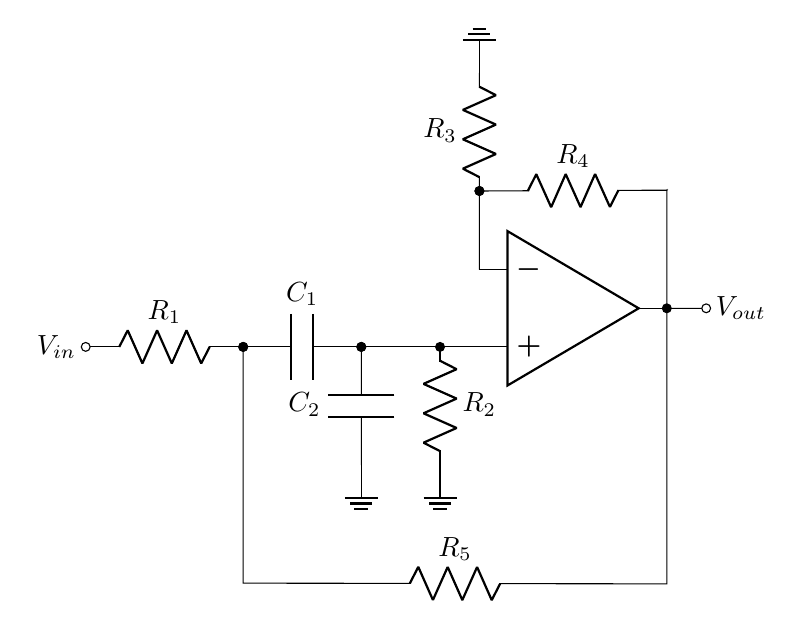
\begin{tikzpicture}
	\node[op amp, yscale=1] (opamp) at (6,-0.5) {};
	\draw ($(opamp.+)+(-5,0)$) node[left] {$V_{in}$} 
	to[R, l=$R_1$, o-*] ($(opamp.+)+(-3,0)$) node (nodebetween1) {}
	to[C, l=$C_1$, *-*] ($(opamp.+)+(-1.5,0)$) node (nodebetween2) {}
	to ($(opamp.+)+(-0.5,0)$) node (nodebetween4) {}
	to[short] (opamp.+);
	\draw (nodebetween2.center) to[C, l_=$C_2$, *-] ($(nodebetween2)+(0,-1.5)$) node [ground] {};
	\draw (nodebetween4.center) to[R, l=$R_2$, *-] ($(nodebetween4)+(0,-1.5)$) node [ground] {};
	\draw (nodebetween1.center) to[short] ($(nodebetween1)+(0,-3)$) 
	to[R, l=$R_5$] ($(opamp.out)+(0,-3.5)$) 
	to[short] (opamp.out);
	\draw (opamp.-) to[short] ($(opamp.-)+(0,1)$) node (nodebetween3) {}
	to[R, l=$R_4$, *-]  ($(opamp.out)+(0,1.5)$) 
	to[short] ($(opamp.out)+(0,1.5)$) 
	to[short] (opamp.out);
	\draw (nodebetween3.center) to[R, l=$R_3$, *-] ($(nodebetween3)+(0,1.5)$) node [ground, yscale=-1] {};
	\draw (opamp.out) to[short, *-o]  ($(opamp.out)+(0.5,0)$) node[right] {$V_{out}$};
\end{tikzpicture}
\end{document}